\documentclass[12pt]{article}

% Standard packages
\usepackage[a4paper, margin=1in]{geometry}
\usepackage{amsmath}
\usepackage{graphicx}
\usepackage{hyperref}

% Packages for code formatting
\usepackage{xcolor}
\usepackage{listings}

% Define colors for Python syntax highlighting
\definecolor{codegreen}{rgb}{0,0.6,0}
\definecolor{codegray}{rgb}{0.5,0.5,0.5}
\definecolor{codepurple}{rgb}{0.58,0,0.82}
\definecolor{backcolour}{rgb}{0.95,0.95,0.92}

% Define the style for the code listing
\lstdefinestyle{mystyle}{
    backgroundcolor=\color{backcolour},
    commentstyle=\color{codegreen},
    keywordstyle=\color{blue},
    numberstyle=\tiny\color{codegray},
    stringstyle=\color{codepurple},
    basicstyle=\footnotesize\ttfamily,
    breakatwhitespace=false,
    breaklines=true,
    captionpos=b,
    keepspaces=true,
    numbers=left,
    numbersep=5pt,
    showspaces=false,
    showstringspaces=false,
    showtabs=false,
    tabsize=4,
    language=Python
}
\lstset{style=mystyle}

\title{EE604: Image Processing \\ Homework 6}
\author{Lohit P Talavar \\ 210564}
\date{\today}

\begin{document}

\maketitle

\section{Python Implementation}

\begin{lstlisting}[caption={Python code for computing filter responses using the integral image.}, label={lst:code}]
import cv2
import numpy as np
import matplotlib.pyplot as plt

def compute_integral_image(image: np.ndarray) -> np.ndarray:
    """
    Computes the integral image of a grayscale image.
    The integral image is padded with a top row and a left column of zeros
    to simplify the calculation of rectangular sums.
    """
    # Pad with a row and column of zeros on the top and left
    padded_image = np.pad(image, ((1, 0), (1, 0)), 'constant')
    # Use cumulative sums along both axes to get the integral image
    return np.cumsum(np.cumsum(padded_image, axis=0), axis=1)

def sum_rect(integral_image: np.ndarray, top_left: tuple, height: int, width: int) -> float:
    """
    Calculates the sum of a rectangular region using the integral image.
    Uses the formula: D - B - C + A, where A, B, C, and D are the
    values of the integral image at the corners of the rectangle.
    """
    r, c = top_left
    # Get the four corner values from the integral image
    A = integral_image[r, c]
    B = integral_image[r, c + width]
    C = integral_image[r + height, c]
    D = integral_image[r + height, c + width]
    return D - B - C + A

def apply_filter(integral_image: np.ndarray, rectangles: list, output_shape: tuple, filter_size: tuple = (4, 4)) -> np.ndarray:
    """
    Applies a filter defined by its constituent rectangles to the integral image.
    The filter is slid across the entire image to generate a response map.
    """
    filter_h, filter_w = filter_size
    output_h, output_w = output_shape
    response_map = np.zeros((output_h, output_w), dtype=np.float64)

    # Slide the filter over each possible location in the image
    for r in range(output_h):
        for c in range(output_w):
            response = 0
            # For each rectangle in the filter's definition...
            for (y_off, x_off, h, w, weight) in rectangles:
                # Calculate the sum of pixels in that rectangle
                rect_sum = sum_rect(integral_image, (r + y_off, c + x_off), h, w)
                # Add the weighted sum to the total response
                response += rect_sum * weight
            response_map[r, c] = response
    return response_map

# --- Main Execution ---

# 1. Load the image in grayscale
image_path = 'iitk_0bcd2f00-d737-4e46-9e60-01ffffe1ea81.png'
image = cv2.imread(image_path, cv2.IMREAD_GRAYSCALE)
image = image.astype(np.float64)

# 2. Compute the integral image
integral_img = compute_integral_image(image)

# 3. Define the six 4x4 filters
# Each rectangle is (y_offset, x_offset, height, width, weight)
# White = +1, Gray = -1
rects_f1 = [(0, 0, 2, 4, -1), (2, 0, 2, 4, 1)]
rects_f2 = [(0, 0, 4, 2, -1), (0, 2, 4, 2, 1)]
rects_f3 = [(0, 0, 1, 4, -1), (1, 0, 2, 4, 1), (3, 0, 1, 4, -1)]
rects_f4 = [(0, 0, 4, 1, -1), (0, 1, 4, 2, 1), (0, 3, 4, 1, -1)]
rects_f5 = [(0, 0, 2, 2, -1), (0, 2, 2, 2, 1), (2, 0, 2, 2, 1), (2, 2, 2, 2, -1)]
rects_f6 = [(0, 0, 2, 4, 1), (2, 0, 2, 4, -1)]

all_filters = {
    "Filter 1 (Horiz. Edge)": rects_f1, "Filter 2 (Vert. Edge)": rects_f2,
    "Filter 3 (Horiz. Line)": rects_f3, "Filter 4 (Vert. Line)": rects_f4,
    "Filter 5 (Checkerboard)": rects_f5, "Filter 6 (Inv. Horiz. Edge)": rects_f6,
}

# 4. Calculate output dimensions and apply filters
filter_size = (4, 4)
img_h, img_w = image.shape
output_h = img_h - filter_size[0] + 1
output_w = img_w - filter_size[1] + 1
output_shape = (output_h, output_w)

responses = {}
for name, rects in all_filters.items():
    responses[name] = apply_filter(integral_img, rects, output_shape, filter_size)

# 5. Display and save the results
fig, axes = plt.subplots(4, 2, figsize=(10, 16))
axes = axes.ravel()
axes[0].imshow(image, cmap='gray')
axes[0].set_title('Original Image')
axes[0].axis('off')
for i, (name, response_map) in enumerate(responses.items()):
    ax = axes[i + 1]
    im = ax.imshow(response_map, cmap='gray')
    ax.set_title(name)
    ax.axis('off')
for i in range(len(responses) + 1, len(axes)):
    axes[i].axis('off')
plt.tight_layout()
plt.savefig('Figure_1.png')
plt.show()
\end{lstlisting}

% \newpage
\section{Input}

\begin{figure}[h!]
    \centering
    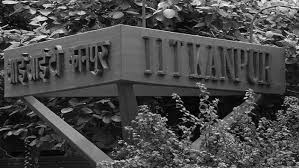
\includegraphics[width=\textwidth]{iitk_0bcd2f00-d737-4e46-9e60-01ffffe1ea81.png}
    \caption{Original image}
    \label{fig:output}
\end{figure}
\section{Output}

\begin{figure}[h!]
    \centering
    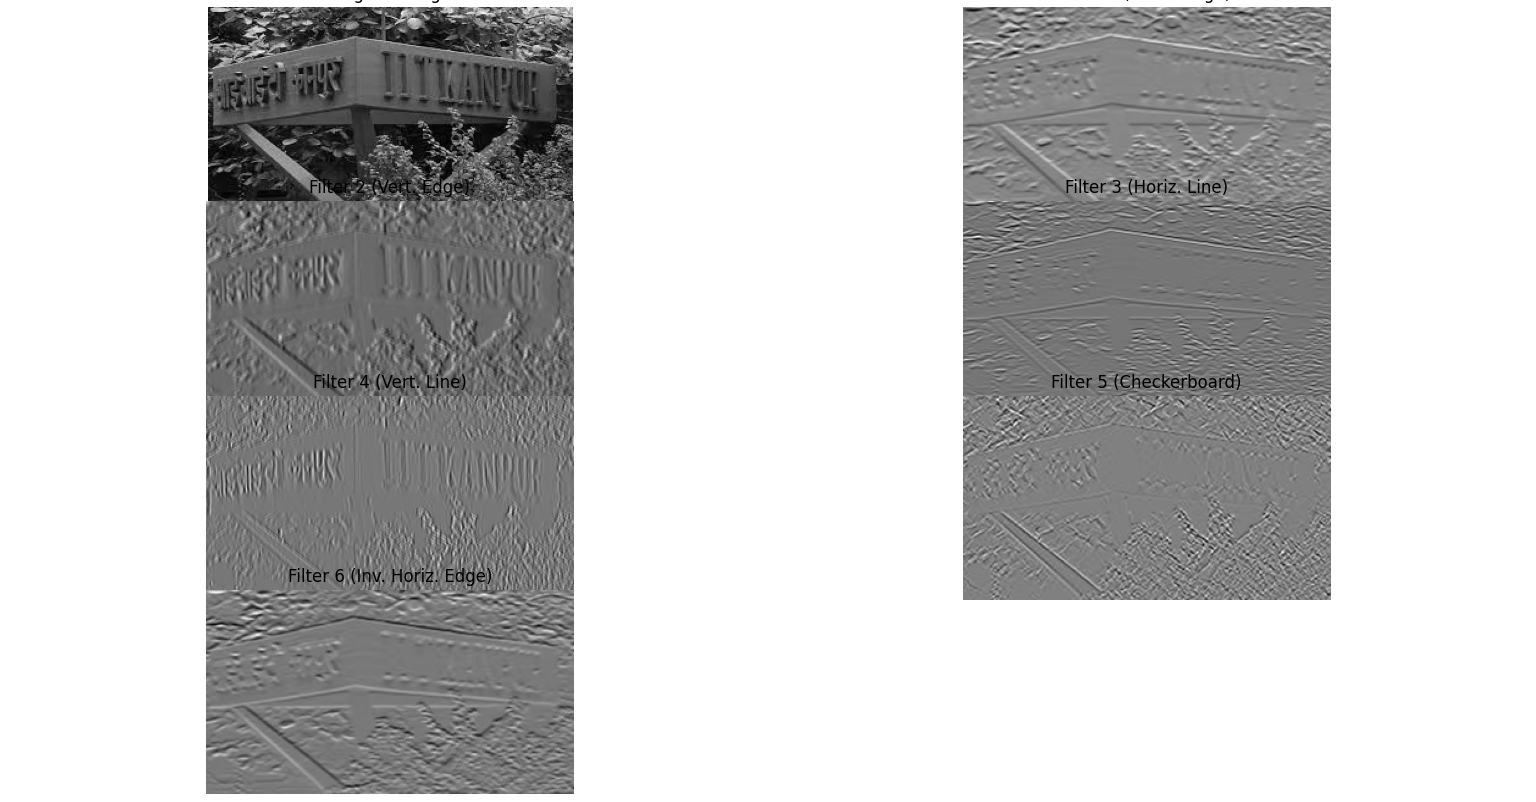
\includegraphics[width=\textwidth]{Figure_1.png}
    \caption{Output showing the original image and the response maps for the six filters.}
    \label{fig:output}
\end{figure}

\end{document}